%%%%%%%%%%%%%%%%%%
%%%%%%%%%%%%%%%%%%
%
%\begin{frame}
%\shiftedframetitle{3. Tools}

%\begin{figure}
%\begin{minipage}{0.15\linewidth}
%%\vspace{-2.5cm}
%\begin{tcolorbox}[title=\centering SWE solver\\2D,colframe=TUMDarkBlue,
%colback=TUMDarkBlue!30]
%\addtolength{\leftmargini}{-1.5em}
%\begin{itemize}
%\setlength{\itemsep}{5ex}
%%\addtolength{\itemindent}{-2em} 
%\vspace{0.5cm}
%\item Riemann Solver $\rightarrow$ \textit{F-Wave}
%\item Developed at SCCS
%\item Written in C++
%\end{itemize}
%\end{tcolorbox}
%\end{minipage}
%\begin{minipage}{0.08\linewidth}
%%\vspace{-3.25cm}
%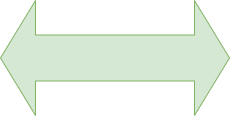
\includegraphics[width=1\textwidth]{Resources/Images/arrow2.png}
%\end{minipage}
%\begin{minipage}{0.46\linewidth}
%%\vspace{-2.5cm}
%\includegraphics[width=1\textwidth]{Resources/Images/imagesThesis/preCICE_overview.png}
%\end{minipage}
%\begin{minipage}{0.08\linewidth}
%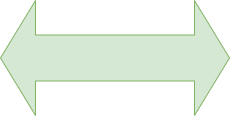
\includegraphics[width=1\textwidth]{Resources/Images/arrow2.png}
%\end{minipage}
%\begin{minipage}{0.21\linewidth}
%%\vspace{-2.5cm}
%\begin{tcolorbox}[title=\centering interFoam\\3D, colframe=TUMOrange,
%colback=TUMOrange!30] 
%%\settowidth{\leftmargini}{\usebeamertemplate{itemize item}}
%\addtolength{\leftmargini}{-1.5em}
%\begin{itemize}
%\setlength{\itemsep}{10ex}
%%\addtolength{\itemindent}{-2em} 
%\vspace{0.5cm}
%\item OpenFOAM Multiphase Navier-Stokes Solver
%\item Volume of Fluid $\rho=\alpha\rho_1 + (1-\alpha)\rho_2$
%\end{itemize}
%\end{tcolorbox}
%\end{minipage}
%\end{figure}

%\begin{minipage}{1\textwidth}
%\begin{itemize}
%\addtolength{\itemindent}{-1em} 
%\item<2->[] \begin{tcolorbox}[colframe=TUMGreen,
%colback=TUMGreen!30] 
%\centering
%\textbf{A flexible approach to 2D - 3D coupling of a Shallow Water Equations solver to OpenFOAM}
%\end{tcolorbox}
%\end{itemize}
%\end{minipage}
%\begin{figure}
%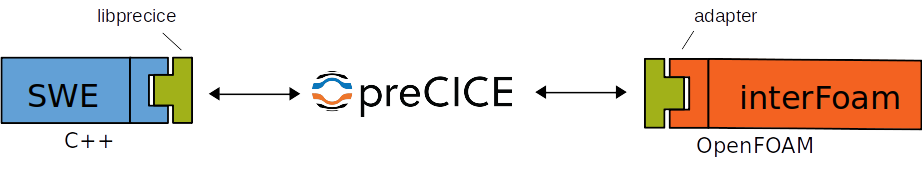
\includegraphics[scale=0.5]{Resources/Images/pash.png}
%\end{figure}
%\end{frame}




%\end{itemize}
%
%\textbf{preCICE - \small{Open-Source coupling library for partitioned multi-physics simulations}}
%\begin{itemize}
%\vspace{5pt}
%\item coupling \& mapping
%\begin{itemize}
%\item[] multi-physics \myCRed{partitioned} problems
%%\item[] two domains on \textit{same} or \textit{different} dimensions/so
